\chapter{MARCO TEÓRICO}

\subsection*{Resumen}
\textit{En este capítulo se desarrollan los fundamentos teóricos y conceptuales que sustentan el diseño del protocolo de votación electrónica post-cuántica. Se describen en primer lugar las propiedades de seguridad que debe cumplir un sistema electoral digital y las vulnerabilidades que presenta la criptografía clásica frente a las computadoras cuánticas. Posteriormente, se explican de manera progresiva los conceptos de retículos geométricos, el problema de aprendizaje con errores (LWE) y los estándares criptográficos post-cuánticos del NIST (FIPS 203, FIPS 204 y FIPS 202). Finalmente, se exponen los principios de la verificación formal de protocolos con Tamarin Prover y la metodología de ingeniería web basada en UML (UWE) utilizada para el diseño de la aplicación web.}

% =============================================================================

\section{Votación Electrónica y Propiedades de Seguridad}
% =============================================================================

Un sistema de votación electrónica se define formalmente como el conjunto de procedimientos criptográficos, protocolos de comunicación, arquitecturas de software e infraestructuras de cómputo que permiten la acreditación de electores, la emisión confidencial del sufragio, su registro inmutable, su transmisión segura y el cómputo final de resultados mediante medios digitales (Gritzalis, 2002; Volkamer, 2009). 

A diferencia de los sistemas de información transaccionales convencionales ---tales como las plataformas bancarias, el comercio electrónico o la gestión gubernamental en línea---, el diseño de un sistema electoral digital enfrenta requerimientos de seguridad estrictamente antagónicos: debe garantizar simultáneamente la autenticidad e identificación inequívoca del ciudadano en la fase de acceso, y la desvinculación estricta y permanente entre dicha identidad y el contenido de su papeleta en las fases de custodia y escrutinio (Chaum, 1981; Chaum, 1982; Benaloh, 1987).

\subsection{Evolución Histórica y Enfoques Criptográficos en Sistemas Electorales}

Desde la formulación de los primeros esquemas criptográficos en la década de 1980, la literatura especializada ha explorado tres grandes paradigmas para resolver la tensión entre anonimato y auditabilidad:

\begin{enumerate}
	\item \textbf{Redes de Mezcla (\textit{Mix-Nets}):} Propuestas originalmente por David Chaum (1981), se basan en una secuencia de servidores independientes denominados \textit{mixes}. Cada servidor recibe un lote de boletas cifradas con capas sucesivas de criptografía de clave pública, aplica una permutación aleatoria secreta a los elementos y remueve una capa de cifrado antes de retransmitirlos al siguiente nodo. Si al menos un servidor de la cadena es honesto, se destruye la correlación temporal y espacial entre el emisor y el mensaje saliente. Variantes modernas incorporan pruebas de conocimiento cero de permutación correcta (\textit{verifiable shuffles}) (Neff, 2001; Cortier et al., 2014).
	\item \textbf{Cifrado Homomórfico y Pruebas de Conocimiento Cero ($ZKP$):} Introducido en el ámbito electoral por Benaloh (1987) y formalizado por Cramer, Gennaro y Schoenmakers (1997), este enfoque permite computar operaciones algebraicas sobre los votos directamente en su forma cifrada. Empleando criptosistemas aditivamente homomórficos (como Paillier o ElGamal exponencial), las autoridades multiplican los textos cifrados para obtener el cifrado de la suma de los votos, descifrando únicamente el resultado final consolidado sin abrir jamás una boleta individual.
	\item \textbf{Firmas Ciegas (\textit{Blind Signatures}):} Diseñadas por Chaum (1988) y aplicadas al sufragio por Fujioka, Okamoto y Ohta (1992) en el seminal protocolo FOO. El votante introduce su papeleta dentro de un ``sobre ciego digital'' mediante un factor de enmascaramiento aleatorio; la autoridad firma el sobre opaco certificando que el elector está empadronado, y posteriormente el votante retira la máscara, obteniendo una credencial válidamente firmada que puede depositar anónimamente en el ánfora a través de un canal desvinculado.
\end{enumerate}

\subsection{Taxonomía Formal de las Propiedades de Seguridad Electoral}

La doctrina de seguridad de la información electoral clasifica los requisitos que debe satisfacer cualquier protocolo comicial en cuatro dimensiones fundamentales (Volkamer, 2009; Bernhard et al., 2012; Cortier et al., 2014):

\subsubsection{Confidencialidad y Privacidad del Sufragio (\textit{Ballot Secrecy})}
El secreto del voto constituye un principio democrático consagrado internacionalmente. Desde la teoría criptográfica, la confidencialidad exige que ningún actor ---incluyendo los administradores de la red, los proveedores de infraestructura y las propias autoridades electorales coludidas--- sea capaz de asociar la identidad de un votante con la opción política seleccionada (Bernhard et al., 2012).

En la literatura avanzada se distinguen tres niveles crecientes de privacidad:
\begin{itemize}
	\item \textbf{Secreto Simple (\textit{Ballot Privacy}):} Ningún observador pasivo o activo del tráfico de red puede deducir la preferencia contenida en la boleta con una ventaja estadística superior a la de una estimación aleatoria.
	\item \textbf{Libertad de Recibo (\textit{Receipt-Freeness}):} Formalizada por Benaloh y Tuinstra (1994) y Delaune, Kremer y Ryan (2009), establece que el sistema no debe entregar al votante ningún elemento o comprobante que le permita demostrar fehacientemente a un tercero por quién votó. Esta propiedad neutraliza de raíz los esquemas comerciales de compra y venta de votos (\textit{vote buying}).
	\item \textbf{Resistencia a la Coacción (\textit{Coercion Resistance}):} Formulada por Juels, Catalano y Jakobsson (2010), constituye la garantía más exigente: asegura que el votante pueda resistir la extorsión o intimidación directa de un coactor, incluso en escenarios donde el coactor le ordene compartir sus credenciales secretas, le instruya qué votar o presencie físicamente la pantalla del dispositivo durante la emisión.
\end{itemize}

\subsubsection{Verificabilidad de Extremo a Extremo (\textit{End-to-End Verifiability, E2E-V})}
A diferencia de los sistemas de cómputo cerrados en los que la sociedad debe depositar un ``acto de fe ciega'' en los ingenieros de software o en los fabricantes de hardware, los protocolos criptográficos modernos implementan el principio de \textbf{Verificabilidad de Extremo a Extremo} (Chaum, 2004; Adida, 2008; Ryan et al., 2009). Formalizada por Cortier, Delaune e Issarny (2014), la verificabilidad E2E-V exige el cumplimiento concurrente de tres propiedades matemáticas auditables:

\begin{enumerate}
	\item \textbf{Emitido según la intención (\textit{Cast-as-Intended}):} El votante tiene la certeza técnica de que el criptograma generado en su terminal refleja fielmente la opción que marcó en pantalla, sin que un programa malicioso (\textit{malware}) en el navegador o en la cabina haya sustituido su decisión. Esto se resuelve comúnmente mediante el mecanismo interactivo de auditoría \textit{Benaloh Challenge} (\textit{cast-or-spoil}) (Benaloh, 1987) o mediante esquemas de comprobación visual criptográfica (Chaum, 2004).
	\item \textbf{Registrado según lo emitido (\textit{Recorded-as-Cast}):} El votante recibe un comprobante público o código de seguimiento determinista (como un hash inmutable) que le permite verificar en un tablero o boletín de acceso abierto (\textit{public bulletin board}) que su papeleta cifrada fue recibida e incorporada formalmente en la urna digital sin alteraciones ni omisiones.
	\item \textbf{Contabilizado según lo registrado (\textit{Tallied-as-Recorded}):} Cualquier ciudadano, fiscal partidario u observador internacional puede auditar matemáticamente el escrutinio final a partir del conjunto íntegro de boletas publicadas en el boletín, constatando que el cómputo oficial deriva de forma exacta y no corrompida de las papeletas archivadas en la urna, sin necesidad de confiar en la honestidad de las autoridades.
\end{enumerate}

\subsubsection{Elegibilidad, Unicidad del Sufragio y No Repudio}
\begin{itemize}
	\item \textbf{Elegibilidad (\textit{Eligibility}):} Únicamente los ciudadanos legalmente empadronados y habilitados por la Autoridad de Registro pueden inyectar un voto válido en el sistema (Sampigethaya y Poovendran, 2006).
	\item \textbf{Unicidad (\textit{One-Person One-Vote / Unreusability}):} Cada elector habilitado puede emitir exactamente un voto admisible. Cualquier intento deliberado o accidental de depositar papeletas adicionales debe ser detectado y neutralizado en tiempo real por el servidor de recepción (Fujioka et al., 1992).
	\item \textbf{No Repudio e Integridad de la Emisión:} El sufragio legítimo debe incorporar una vinculación criptográfica irrefutable (mediante firma digital) que impida al elector desconocer la autoría de una emisión válida, protegiendo al sistema ante impugnaciones fraudulentas posteriores (Cramer et al., 1997).
\end{itemize}

\subsubsection{Robustez y Tolerancia a Fallos (\textit{Robustness})}
El protocolo debe ser capaz de culminar el proceso comicial y generar un resultado incontrovertible incluso ante la presencia de votantes maliciosos que envíen paquetes corrompidos, la caída transitoria de enlaces de telecomunicaciones o la deserción de un subconjunto de autoridades electorales (Cramer et al., 1997; Chevallier-Mames et al., 2010).

\subsection{La Paradoja de la Votación Electrónica frente a la Banca Digital}

Diversos autores (Saltman, 2006; Volkamer, 2009; Bernhard et al., 2017) han destacado la singular complejidad conceptual del voto digital frente a otras aplicaciones críticas de la computación distribuida:

\begin{quote}
	\small\textit{``En una transacción bancaria o de comercio electrónico, la seguridad se basa en la correlación perfecta y auditable: el cliente exige un recibo firmado que documente con la máxima precisión su identidad, la fecha exacta y el monto transferido, de modo que dicho comprobante pueda emplearse como prueba ante una disputa legal. En la votación democrática, por el contrario, la ley electoral prohíbe de manera terminante entregarle al ciudadano un recibo que exponga su elección en claro, pues dicho comprobante se transformaría en el instrumento predilecto para la compra de votos, el clientelismo y la coacción patronal o política.''} (Adaptado de Saltman, 2006; Volkamer, 2009).
\end{quote}

Esta aparente contradicción ---demostrar matemáticamente que un voto fue fielmente registrado y escrutado, sin entregar ningún comprobante que delate el contenido de la elección--- es el desafío central que la criptografía asimétrica moderna resuelve mediante el uso de funciones unidireccionales con trampa, compromisos criptográficos y resúmenes hash públicos deterministas.

\subsection{Lecciones de Vulnerabilidades en Protocolos Abiertos (Helios y Belenios)}

La viabilidad práctica de los protocolos verificables de extremo a extremo quedó demostrada con el desarrollo de plataformas de código abierto como \textbf{Helios Voting} (Adida, 2008), utilizada extensamente en elecciones académicas internacionales (incluyendo la Universidad de Lovaina y la Universidad de Princeton), y su sucesora europea \textbf{Belenios} (Cortier et al., 2019).

No obstante, la literatura contemporánea ha evidenciado que la robustez matemática aislada de las primitivas criptográficas no garantiza por sí misma la seguridad del sistema si existen deficiencias en el diseño lógico de las interacciones. Baloglu, Bursuc, Mauw y Pang (2021) aplicaron técnicas avanzadas de verificación formal automatizada sobre Helios y Belenios, identificando vulnerabilidades sutiles que habían eludido más de una década de auditorías manuales:
\begin{itemize}
	\item Ataques de sustitución y maleabilidad de textos cifrados (\textit{ballot-stuffing / replay}), en los que un adversario interceptaba boletas válidas y las reinyectaba bajo identificadores artificiales alterando la distribución estadística del conteo.
	\item Fugas de privacidad derivadas de la sincronización de credenciales institucionales compartidas entre la autoridad de autenticación y los servidores de depósito.
\end{itemize}

Los hallazgos de Baloglu et al. (2021) establecieron una conclusión metodológica determinante para la ciencia de la computación: los protocolos de votación no deben ser validados únicamente mediante inspección empírica o pruebas convencionales de software, sino a través de \textbf{modelos de verificación formal basados en lógica matemática y reescritura de términos}, sometidos a las condiciones adversariales más hostiles posibles.

\subsection{El Principio de la Función Unidireccional con Trampa}

Desde la perspectiva criptográfica, la seguridad de cualquier esquema de votación electrónica descansa sobre el concepto de \textit{funciones unidireccionales con trampa} (\textit{trapdoor one-way functions}) (Diffie y Hellman, 1976). Una función $f: X \to Y$ se considera unidireccional si calcular la imagen $y = f(x)$ es computacionalmente eficiente (tiempo polinomial), pero invertir la operación para hallar una preimagen $x \in f^{-1}(y)$ es intratable para cualquier algoritmo clásico eficiente, a menos que se disponga de una información privilegiada adicional denominada \textit{trampa secreta} (\textit{trapdoor}).

\begin{figure}[htbp]
	\centering
	\begin{tikzpicture}[
		scale=0.9,
		node distance=1.1cm,
		cbox/.style={rectangle, draw=black, fill=white, line width=0.8pt, rounded corners=1.5pt, align=center, font=\footnotesize, inner sep=5pt}
	]
		\node (in) [cbox, text width=2.8cm] {\textbf{Mensaje / Voto}\\$x \in X$};
		\node (proc) [cbox, right=of in, text width=3.4cm] {\textbf{Cálculo Criptográfico}\\$y = f(x)$ \ (Polinomial)};
		\node (out) [cbox, right=of proc, text width=2.8cm] {\textbf{Criptograma / Boleta}\\$y \in Y$};
		
		\draw[-{Latex[length=2mm, width=1.5mm]}, line width=0.8pt] (in) -- (proc);
		\draw[-{Latex[length=2mm, width=1.5mm]}, line width=0.8pt] (proc) -- (out);
		
		\draw[-{Latex[length=2mm, width=1.5mm]}, line width=0.7pt, dashed] (out.north) to[bend right=40] 
		node[midway, above, font=\scriptsize\itshape] {Inversión intratable sin trampa} (in.north);
		
		\node (trap) [cbox, below=0.85cm of proc, text width=4.0cm] {\textbf{Trampa Secreta (Clave Privada)}\\Permite calcular $x = f^{-1}(y)$ en tiempo eficiente};
		\draw[-{Latex[length=2mm, width=1.5mm]}, line width=0.8pt] (trap) -- (proc);
	\end{tikzpicture}
	\caption{Principio estructural de una función unidireccional con trampa.}
	\label{fig:trapdoor_func}
	\par\vspace{3pt}{\footnotesize\textit{Fuente: Adaptado de Diffie y Hellman (1976).}}
\end{figure}

En un protocolo de votación, la papeleta es transformada mediante la clave pública electoral en un criptograma indescifrable para el canal, mientras que la autoridad de cómputo utiliza la clave privada como trampa matemática para la apertura legítima al cierre de la jornada electoral.

% =============================================================================
\section{Criptografía de Clave Pública Clásica y su Vulnerabilidad Cuántica}
% =============================================================================

Los esquemas criptográficos de clave pública empleados históricamente de forma predominante en sistemas de votación electrónica ---entre ellos RSA y ECDSA--- sustentan su seguridad computacional en dos problemas aritméticos fundamentales: la factorización de enteros grandes y el logaritmo discreto sobre grupos finitos o curvas elípticas.

\subsection{El Mecanismo Clásico de RSA}

Propuesto por Rivest, Shamir y Adleman (1978), el esquema RSA basa su asimetría en que la multiplicación de dos números primos grandes $p$ y $q$ es trivialmente calculable en milisegundos, mientras que la operación inversa ---factorizar el módulo compuesto $N = p \cdot q$--- requiere un esfuerzo computacional que crece de forma subexponencial con el algoritmo clásico más avanzado conocido (la Criba General del Cuerpo de Números, GNFS).

La función de cifrado de un mensaje $m \in \mathbb{Z}_N$ bajo el exponente público $e$ se define como:
\begin{equation}
	c \equiv m^e \pmod N
\end{equation}
Para descifrar, el receptor legítimo requiere calcular el exponente privado $d \equiv e^{-1} \pmod{\phi(N)}$, donde $\phi(N) = (p-1)(q-1)$ corresponde a la función totiente de Euler:
\begin{equation}
	m \equiv c^d \pmod N
\end{equation}
Un atacante que intente deducir $d$ únicamente a partir de la información pública $(e, N)$ se enfrenta a la necesidad insalvable de factorizar $N$. Para una clave estándar de RSA-2048, el esfuerzo computacional clásico demandaría miles de años de cómputo en supercomputadoras actuales.

\subsection{El Algoritmo Cuántico de Shor}

La seguridad de RSA y de los esquemas basados en curvas elípticas colapsa teóricamente frente al advenimiento de una computadora cuántica de escala suficiente debido al algoritmo de factorización y logaritmo discreto formulado por Peter Shor (1997).

Shor demostró que el problema de factorizar un entero compuesto $N$ puede reducirse matemáticamente al problema de encontrar el \textit{período} $r$ de una función periódica definida sobre el grupo multiplicativo $(\mathbb{Z}_N)^*$:
\begin{equation}
	f(x) = a^x \pmod N
\end{equation}
donde $a$ es un entero coprimo con $N$. Dicha función es estrictamente periódica: satisface $f(x + r) = f(x)$, con $a^r \equiv 1 \pmod N$. Si el período $r$ es par, se cumple:
\begin{equation}
	a^r - 1 \equiv (a^{r/2} - 1)(a^{r/2} + 1) \equiv 0 \pmod N
\end{equation}
Al calcular el máximo común divisor mediante el algoritmo euclídeo clásico:
\begin{equation}
	\gcd(a^{r/2} - 1, N) \quad \text{y} \quad \gcd(a^{r/2} + 1, N)
\end{equation}
se obtienen de forma no trivial los factores primos $p$ y $q$ de $N$.

Mientras que una computadora clásica requiere tiempo exponencial o subexponencial para hallar dicho período evaluando combinaciones punto por punto, una computadora cuántica ejecuta la \textbf{Transformada Cuántica de Fourier} (\textit{Quantum Fourier Transform}, QFT). La QFT aprovecha el fenómeno de superposición cuántica y la interferencia destructiva para concentrar las amplitudes de probabilidad en las frecuencias resonantes correspondientes al período $r$, resolviendo la búsqueda en tiempo polinomial estricto $\mathcal{O}((\log N)^3)$.

\subsection{La Amenaza ``Cosechar Ahora, Descifrar Después''}

La vulnerabilidad cuántica no representa únicamente un riesgo futuro, sino una amenaza operativa inmediata clasificada por las agencias de estandarización técnica bajo el término \textit{Harvest Now, Decrypt Later} (HNDL; cosechar ahora para descifrar después) (Chen et al., 2016). Un adversario puede interceptar y almacenar pasivamente las boletas y credenciales electorales transmitidas en los procesos democráticos contemporáneos cifrados con RSA o ECDSA. Una vez que se cuente con un procesador cuántico tolerante a fallos (\textit{Fault-Tolerant Quantum Computer}, FTQC), dicho registro histórico podrá ser descifrado retroactivamente, vulnerando permanentemente la confidencialidad del voto de los electores.

% =============================================================================
\section{Fundamentos Geométricos de la Criptografía Basada en Retículos}
% =============================================================================

Frente a la debilidad de las estructuras cíclicas multiplicativas, la criptografía post-cuántica recurre a problemas de álgebra lineal geométrica sobre espacios euclídeos discretos: los \textbf{retículos} (\textit{lattices}).

\subsection{Definición Formal de Retículo}

Dado un conjunto de $k$ vectores linealmente independientes $\mathbf{B} = \{\mathbf{b}_1, \mathbf{b}_2, \dots, \mathbf{b}_k\} \subset \mathbb{R}^m$, el retículo $\Lambda$ generado por la base $\mathbf{B}$ se define como el conjunto de todas las combinaciones lineales con coeficientes enteros (Micciancio y Goldwasser, 2002):
\begin{equation}
	\Lambda = \mathcal{L}(\mathbf{B}) = \left\{ \sum_{i=1}^{k} z_i \mathbf{b}_i \;\middle|\; z_i \in \mathbb{Z} \right\}
\end{equation}
El entero $k$ se denomina el \textit{rango} del retículo y $m$ su \textit{dimensión}. Cuando $k = m$, el retículo se considera de rango completo.

\begin{figure}[htbp]
	\centering
	\begin{tikzpicture}[scale=0.88]
		% Puntos del retículo como puntos analógicos nítidos
		\foreach \x in {-2,...,3} {
			\foreach \y in {-2,...,2} {
				\coordinate (P) at ({\x*1.5 + \y*0.7}, {\x*0.4 + \y*1.8});
				\fill[black] (P) circle (1.3pt);
			}
		}
		\coordinate (O) at (0,0);
		\node[below left, font=\scriptsize] at (O) {$\mathbf{0}$};
		
		% Vectores de la base
		\draw[-{Latex[length=2.2mm, width=1.5mm]}, line width=0.9pt] (O) -- (1.5, 0.4) 
		node[midway, below right, font=\footnotesize] {$\mathbf{b}_1$};
		\draw[-{Latex[length=2.2mm, width=1.5mm]}, line width=0.9pt] (O) -- (0.7, 1.8) 
		node[midway, above left, font=\footnotesize] {$\mathbf{b}_2$};
		
		% Punto CVP perturbado por ruido
		\coordinate (Closest) at ({1*1.5 + 1*0.7}, {1*0.4 + 1*1.8});
		\coordinate (T) at ({1*1.5 + 1*0.7 + 0.35}, {1*0.4 + 1*1.8 + 0.45});
		
		\fill[black] (T) circle (1.8pt) node[above right, font=\scriptsize] {$\mathbf{t} = \mathbf{v} + \mathbf{e}$};
		\draw[-{Latex[length=1.8mm, width=1.2mm]}, line width=0.7pt] (Closest) -- (T) 
		node[midway, right, font=\tiny\itshape] {$\mathbf{e}$};
		\draw[line width=0.6pt, dotted] (Closest) circle (7pt);
	\end{tikzpicture}
	\caption{Retículo bidimensional con vectores base y punto objetivo perturbado por ruido en el problema CVP.}
	\label{fig:reticulo_2d}
	\par\vspace{3pt}{\footnotesize\textit{Fuente: Elaboración propia.}}
\end{figure}

\subsection{Bases Cortas (Buenas) versus Bases Distorsionadas (Malas)}

Una propiedad geométrica central es que un mismo retículo puede ser generado por infinitas matrices base distintas vinculadas mediante matrices unimodulares $\mathbf{U} \in \mathbb{Z}^{k \times k}$ tales que $\det(\mathbf{U}) = \pm 1$:
\begin{equation}
	\mathbf{B}' = \mathbf{B} \cdot \mathbf{U}
\end{equation}
\begin{itemize}
	\item \textbf{Base ``Buena'' (ortogonal y corta):} Sus vectores poseen normas euclídeas reducidas y ángulos cercanos a $90^\circ$. Permite delimitar celdas fundamentales convexas y resolver problemas de cercanía mediante redondeo simple de coordenadas.
	\item \textbf{Base ``Mala'' (larga y altamente sesgada):} Formada por vectores de gran magnitud y direcciones casi colineales. Sus celdas fundamentales son hiperparalelepípedos elongados que oscurecen la geometría del retículo.
\end{itemize}

Esta disparidad constituye la base de la puerta trampa en retículos: la clave privada corresponde a una base reducida y corta, mientras que la clave pública consiste en una base algebraicamente equivalente pero distorsionada.

\subsection{Problemas Computacionales Intratables: SVP y CVP}

La seguridad de las construcciones post-cuánticas se fundamenta en la intratabilidad demostrada de dos problemas geométricos en dimensiones elevadas ($n \ge 500$):

\begin{enumerate}
	\item \textbf{Problema del Vector Más Corto (Shortest Vector Problem, SVP):} Dado un retículo $\Lambda$, hallar un vector no nulo $\mathbf{v} \in \Lambda \setminus \{\mathbf{0}\}$ tal que su norma euclídea sea mínima: $\|\mathbf{v}\| = \lambda_1(\Lambda) = \min_{\mathbf{x} \in \Lambda \setminus \{\mathbf{0}\}} \|\mathbf{x}\|$.
	\item \textbf{Problema del Vector Más Cercano (Closest Vector Problem, CVP):} Dado un retículo $\Lambda$ y un vector arbitrario $\mathbf{t} \in \mathbb{R}^m$ que no pertenece al retículo, hallar el punto $\mathbf{v} \in \Lambda$ que minimice la distancia euclídea $\|\mathbf{t} - \mathbf{v}\|$.
\end{enumerate}

Ajtai (1996) estableció una propiedad fundamental para la criptografía: las reducciones \textit{worst-case to average-case}. Esto significa que resolver una instancia típica o aleatoria generada por un esquema criptográfico es tan difícil como resolver la peor instancia posible del problema geométrico sobre retículos. Los algoritmos cuánticos conocidos no ofrecen una ventaja más allá de mejoras polinomiales en el exponente de los algoritmos de reducción de base (como BKZ cuántico), requiriendo tiempo asintótico $\mathcal{O}(2^{c \cdot n})$.

% =============================================================================
\section{Aritmética Modular y el Problema Learning With Errors (LWE)}
% =============================================================================

\subsection{De Ecuaciones Lineales Exactas a Sistemas Ruidosos}

En el anillo de enteros módulo $q$, denotado por $\mathbb{Z}_q = \{0, 1, \dots, q-1\}$, un sistema lineal exacto de la forma:
\begin{equation}
	\mathbf{A} \cdot \mathbf{s} \equiv \mathbf{b} \pmod q
\end{equation}
con $\mathbf{A} \in \mathbb{Z}_q^{m \times n}$, $\mathbf{s} \in \mathbb{Z}_q^n$ y $\mathbf{b} \in \mathbb{Z}_q^m$, puede resolverse de manera determinista mediante eliminación gaussiana en tiempo polinomial $\mathcal{O}(m n^2)$. La linealidad perfecta permite a un observador eliminar incógnitas sistemáticamente mediante combinaciones lineales de filas.

\subsubsection{La Intuición de la Perturbación: Por qué Falla Gauss}
Consideremos la analogía básica del álgebra lineal: despejar un sistema lineal de ecuaciones es equivalente a encontrar la intersección exacta de varios hiperplanos. Si las ecuaciones son exactas, la eliminación gaussiana va pivoteando y restando múltiplos de filas hasta triangular la matriz y despejar cada incógnita limpiamente.

Sin embargo, si a cada ecuación se le inyecta un pequeño vector de perturbación estocástica $\mathbf{e}$:
\begin{equation}
	\mathbf{A} \cdot \mathbf{s} + \mathbf{e} \equiv \mathbf{b} \pmod q
\end{equation}
el método de eliminación gaussiana colapsa de forma estrepitosa: al multiplicar una fila por un escalar para anular un coeficiente de otra fila, el término de error $\mathbf{e}$ también se multiplica y se acumula; a medida que se avanza en las etapas de eliminación, el ruido residual crece de manera exponencial, destruyendo cualquier correlación lineal con la incógnita original. Resolver este sistema ruidoso equivale a encontrar el vector del retículo más cercano al punto perturbado (CVP), problema que carece de algoritmos eficientes tanto clásicos como cuánticos.

\subsection{Formulación de LWE (Regev, 2005)}

Oded Regev (2005) demostró que si cada ecuación lineal es perturbada por un término de error discreto e independiente $\mathbf{e}$, la estructura lineal colapsa:
\begin{equation}
	\mathbf{b} = \mathbf{A} \cdot \mathbf{s} + \mathbf{e} \pmod q
\end{equation}
donde las entradas de $\mathbf{A}$ se eligen uniformemente al azar en $\mathbb{Z}_q$, el vector secreto $\mathbf{s}$ proviene de una distribución pequeña, y el vector de error $\mathbf{e} \in \mathbb{Z}_q^m$ se muestrea a partir de una distribución gaussiana discreta centrada en cero con desviación estándar $\sigma \ll q$.

Existen dos formulaciones de este problema:
\begin{itemize}
	\item \textbf{LWE de Búsqueda (\textit{Search-LWE}):} Recuperar el vector secreto exacto $\mathbf{s} \in \mathbb{Z}_q^n$ a partir de la observación pública $(\mathbf{A}, \mathbf{b})$.
	\item \textbf{LWE de Decisión (\textit{Decision-LWE}):} Distinguir computacionalmente entre muestras genuinas $(\mathbf{A}, \mathbf{A}\mathbf{s} + \mathbf{e})$ y pares uniformemente aleatorios $(\mathbf{A}, \mathbf{u}) \in \mathbb{Z}_q^{m \times n} \times \mathbb{Z}_q^m$.
\end{itemize}

Cuando un atacante intenta aplicar combinaciones lineales tipo Gauss sobre el sistema ruidoso, los términos de error se propagan y multiplican, transformando la señal útil en ruido estocástico incoherente. Regev (2005) probó formalmente que resolver Decision-LWE es tan difícil como resolver aproximaciones cuánticas de problemas clásicos de retículos (GapSVP) en dimensión $n$.

\begin{figure}[htbp]
	\centering
	\begin{tikzpicture}[scale=0.9]
		% Señal periódica clásica
		\begin{scope}[shift={(0,2.2)}]
			\node[font=\footnotesize\bfseries, text=PQCCrimson, align=left] at (4.5, 1.2) 
			{\textbf{Esquemas Clásicos (RSA/ECC):} Estructura periódica $f(x)=a^x \pmod N$ $\to$ Shor la detecta};
			\draw[line width=1.4pt, PQCCrimson, domain=0:9, samples=150] plot (\x, {0.5*sin(\x*180/3.14*1.2)});
			\draw[dashed, PQCAmber, line width=1pt] (0,-0.6) -- (9,-0.6);
			\draw[{Latex[length=2mm]}-{Latex[length=2mm]}, PQCAmber, thick] (0,-0.6) -- (2.62,-0.6) 
			node[midway, below, font=\scriptsize] {Período $r$};
		\end{scope}
		
		% LWE Ruidoso
		\begin{scope}[shift={(0,0)}]
			\node[font=\footnotesize\bfseries, text=PQCGreen, align=left] at (4.5, 1.1) 
			{\textbf{Criptografía de Retículos (LWE):} Datos con ruido aleatorio $\mathbf{e}$ $\to$ Ausencia de período (Inmune a Shor)};
			\foreach \x in {0.2,0.5,...,8.8} {
				\pgfmathsetmacro\yr{(rand)*0.55}
				\draw[line width=1.3pt, PQCGreen!80!black] (\x, 0) -- (\x, \yr);
			}
			\draw[line width=0.8pt, gray!60] (0,0) -- (9,0);
		\end{scope}
	\end{tikzpicture}
	\caption{Comparación estructural: la periodicidad explotada por la Transformada Cuántica de Fourier frente a la dispersión aperiódica del ruido en LWE.}
	\label{fig:shor_vs_lwe}
	\par\vspace{3pt}{\footnotesize\textit{Fuente: Elaboración propia.}}
\end{figure}

% =============================================================================
\section{De Álgebra Matricial a Polinomios: Ring-LWE y Module-LWE}
% =============================================================================

\subsection{El Cuello de Botella de Tamaño en LWE Estándar}

Si bien el problema LWE original explicado en el apartado anterior ofrece una gran seguridad frente a las computadoras cuánticas, presenta un inconveniente práctico cuando se intenta utilizar directamente en Internet: el tamaño excesivo de sus claves públicas.

En el esquema LWE estándar, para alcanzar un nivel de seguridad adecuado se necesita una matriz pública $\mathbf{A}$ de cientos de filas por cientos de columnas (por ejemplo, $768 \times 768$ números enteros). Almacenar y enviar por la red todos esos números de forma individual haría que cada clave pública ocupara varios megabytes de memoria. En un sistema de votación electrónica donde miles de usuarios se conectan simultáneamente desde sus navegadores web, transmitir claves tan pesadas saturaría la red y volvería lento el sistema.

\subsection{El Anillo Cociente Polinomial \texorpdfstring{$R_q$}{Rq}}

Para solucionar el problema del tamaño sin perder seguridad, Lyubashevsky, Peikert y Regev (2010) propusieron reemplazar las grandes matrices de números sueltos por \textbf{polinomios}, dando origen a la variante conocida como \textit{Ring-LWE} (Aprendizaje con Errores sobre Anillos).

En lugar de trabajar con miles de ecuaciones independientes, se agrupan $n$ coeficientes dentro de un solo polinomio. El conjunto donde se realizan estas operaciones se denomina anillo de polinomios y se representa como:
\begin{equation}
	R_q = \mathbb{Z}_q[x] / (x^n + 1)
\end{equation}
donde $n$ es una potencia de dos (en los estándares del NIST se fija siempre en $n = 256$). Así, cualquier elemento $a(x)$ perteneciente a $R_q$ es simplemente un polinomio con $256$ términos, cuyos coeficientes son números enteros entre $0$ y $q-1$:
\begin{equation}
	a(x) = a_0 + a_1 x + a_2 x^2 + \dots + a_{n-1} x^{n-1}, \quad a_i \in \mathbb{Z}_q
\end{equation}
Cuando se suman dos polinomios, simplemente se suman sus coeficientes posición por posición. Sin embargo, cuando se multiplican dos polinomios, aparecen potencias iguales o mayores a $x^n$. Para evitar que el polinomio crezca de tamaño, el anillo $R_q$ aplica una regla de reducción muy sencilla: cada vez que aparece el término $x^n$, se reemplaza por $-1$:
\begin{equation}
	x^n \equiv -1 \pmod{x^n + 1}
\end{equation}
Gracias a esta regla, cualquier potencia que supere el grado $n-1$ vuelve a ingresar por el inicio del polinomio cambiando su signo (por ejemplo, $x^n$ se convierte en $-1$, $x^{n+1}$ se convierte en $-x$, y así sucesivamente), manteniendo siempre una longitud fija de $256$ coeficientes.

\subsubsection{Los Polinomios como Arreglos Circulares y la Transformada NTT}

No es necesario imaginar los polinomios de $R_q$ como expresiones algebraicas abstractas; en la memoria de la computadora, estos objetos funcionan de manera muy concreta a través de tres características:

\begin{enumerate}
	\item \textbf{Representación como vector o arreglo:} En lenguajes como C o Python, un polinomio de $R_q$ se programa como un arreglo unidimensional de exactamente $256$ casillas, donde la casilla $0$ guarda $a_0$, la casilla $1$ guarda $a_1$, hasta llegar a la casilla $255$. En el algoritmo ML-KEM el módulo es $q = 3329$ (por lo que cada casilla cabe en un entero corto de $16$ bits), mientras que en ML-DSA el módulo es $q = 8380417$ (almacenado en enteros de $32$ bits).

	\item \textbf{Rotación circular con cambio de signo:} La regla $x^{256} \equiv -1$ significa que, al multiplicar polinomios, los datos que se desplazan más allá de la última casilla del arreglo (posición $255$) reaparecen automáticamente por la primera casilla (posición $0$) multiplicados por $-1$. De este modo, el arreglo nunca cambia de tamaño ni requiere reservar memoria adicional.

	\item \textbf{Multiplicación rápida mediante la Transformada NTT:} Si dos arreglos de $256$ posiciones se multiplican por el método escolar tradicional (todos contra todos), la computadora debe realizar $256 \times 256 = 65\,536$ multiplicaciones. Para acelerar este cálculo, los estándares post-cuánticos utilizan la \textbf{Transformada Teórica de Números} (NTT). La NTT convierte el polinomio a una representación especial donde multiplicar dos polinomios solo requiere multiplicar casilla por casilla ($256$ operaciones), reduciendo la complejidad de $\mathcal{O}(n^2)$ a $\mathcal{O}(n \log n)$ y logrando que el cifrado del voto tome menos de un milisegundo.
\end{enumerate}

En la Figura \ref{fig:anillo_reduccion} se ilustra la descomposición y reducción ciclotómica en el anillo polinomial $R_q = \mathbb{Z}_q[x]/(x^n + 1)$ mediante el árbol de factorización del Teorema del Resto Chino (CRT) y la transformada rápida NTT.

\begin{figure}[htbp]
	\centering
	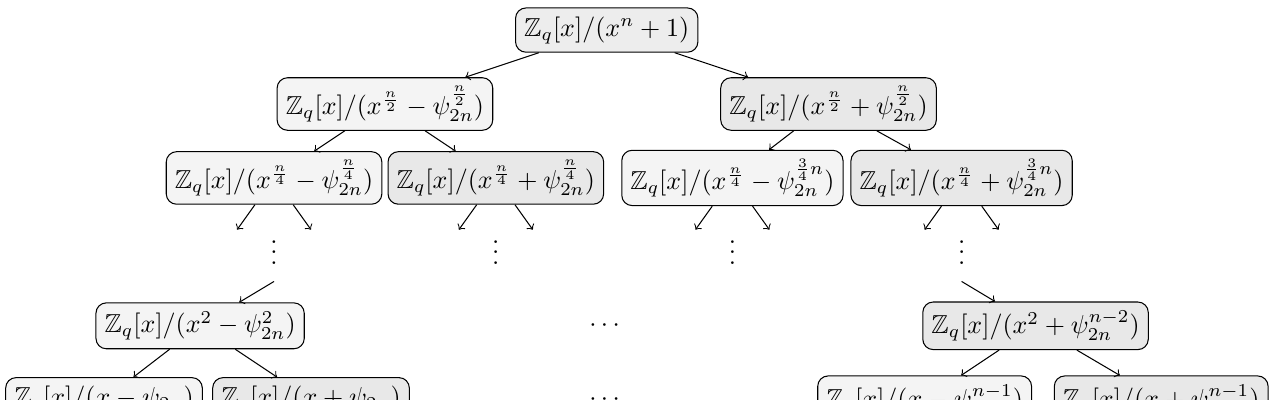
\includegraphics[width=0.90\textwidth,keepaspectratio]{imagenes/autores_cap2/fig_anillo_reduccion_ciclotomica.png}
	\caption{Descomposición y reducción ciclotómica en el anillo polinomial $\mathbb{Z}_q[x]/(x^n + 1)$ mediante transformada NTT.}
	\label{fig:anillo_reduccion}
	\par\vspace{3pt}{\footnotesize\textit{ Liang y Zhao (2022), p. 12.}}
\end{figure}

Como muestra la Figura \ref{fig:anillo_reduccion}, la descomposición jerárquica del polinomio ciclotómico en factores lineales permite calcular multiplicaciones complejas en tiempo $\mathcal{O}(n \log n)$, logrando que un solo polinomio represente una fila completa de la matriz criptográfica y reduciendo drásticamente la cantidad de datos que deben transmitirse entre el navegador del votante y el servidor electoral.

\subsection{Module-LWE: El Compromiso Óptimo de FIPS 203 y 204}

Entre el problema LWE estándar (muy seguro pero con claves demasiado grandes) y el problema Ring-LWE (claves muy pequeñas pero con una estructura fija de un solo polinomio), existe un punto intermedio ideal que fue seleccionado por el NIST para sus estándares oficiales: el problema de \textbf{Aprendizaje con Errores sobre Módulos} o Module-LWE (Langlois y Stehlé, 2015).

La idea de Module-LWE es muy clara: en lugar de usar matrices enormes de números sueltos y en lugar de usar un único polinomio aislado, se utiliza una matriz pequeña de tamaño $k \times k$ donde cada casilla contiene un polinomio de $256$ coeficientes:
\begin{equation}
	\mathbf{s} = \begin{pmatrix} s_1(x) \\ \vdots \\ s_k(x) \end{pmatrix} \in R_q^k, \quad \mathbf{A} \in R_q^{k \times k}
\end{equation}
De este modo, la ecuación con ruido mantiene exactamente la misma forma sencilla:
\begin{equation}
	\mathbf{b} = \mathbf{A} \cdot \mathbf{s} + \mathbf{e} \pmod q
\end{equation}
La gran ventaja de Module-LWE para la ingeniería de software es su flexibilidad. El grado del polinomio se mantiene siempre fijo en $n = 256$ (lo que permite reutilizar las mismas funciones rápidas de multiplicación NTT en el código fuente), y si se desea aumentar el nivel de seguridad del sistema, basta con cambiar el tamaño $k$ de la matriz (por ejemplo, usar $k = 2$ para seguridad básica, $k = 3$ para seguridad intermedia como en ML-KEM-768, o $k = 4$ para seguridad máxima). Con $k = 3$ y $n = 256$, el sistema opera sobre un retículo de $3 \times 256 = 768$ dimensiones utilizando claves compactas de apenas un kilobyte.

% =============================================================================

\section{Mecanismo de Encapsulamiento de Claves ML-KEM (FIPS 203)}
% =============================================================================

En agosto de 2024, el NIST (2024a) publicó el estándar oficial \textbf{FIPS 203}, el cual define el algoritmo de encapsulamiento de claves basado en retículos modulares \textbf{ML-KEM}, originado en el proyecto CRYSTALS-Kyber. Este estándar constituye el mecanismo principal a nivel mundial para proteger la confidencialidad de la información frente a computadoras cuánticas.

\subsection{Concepto de KEM en Votación Electrónica}

Cuando se estudia criptografía por primera vez, suele pensarse que la clave pública sirve para cifrar directamente archivos o mensajes largos. Sin embargo, en la práctica informática moderna se utiliza una técnica mucho más eficiente denominada \textbf{Mecanismo de Encapsulamiento de Claves} (KEM).

El funcionamiento de un KEM puede explicarse mediante una analogía cotidiana: supóngase que el votante desea enviar su boleta electoral dentro de una caja fuerte muy rápida y ligera (cifrado simétrico AES-256-GCM), para lo cual inventa en ese instante una llave secreta única $K$ de $256$ bits. El problema es cómo hacer llegar esa llave $K$ a la Autoridad de Conteo a través de Internet sin que ningún atacante la copie en el camino.

Para resolverlo, el algoritmo ML-KEM no cifra el voto directamente, sino que ``encapsula'' (envuelve) esa llave simétrica $K$ utilizando la clave pública post-cuántica de la autoridad electoral, produciendo una cápsula cifrada $c$. De este modo, el votante cifra su voto con la llave $K$ mediante AES-256-GCM y adjunta la cápsula $c$. Al final de la elección, solo la Autoridad de Conteo posee la clave privada necesaria para abrir la cápsula $c$, recuperar la llave $K$ y leer el contenido del voto.

\subsection{Fases del Protocolo ML-KEM}

El funcionamiento de ML-KEM se compone de tres pasos secuenciales bien definidos: generación de claves, encapsulamiento y desencapsulamiento. En la Figura \ref{fig:kem_flow} se presenta el diagrama general de interacción entre la autoridad electoral y la terminal del votante.

\begin{figure}[!htbp]
	\centering
	\begin{tikzpicture}[
		pbox/.style={rectangle, draw=black, fill=white, line width=0.8pt, rounded corners=1.5pt, text width=3.7cm, align=center, font=\footnotesize\rmfamily, inner sep=5pt},
		decbox/.style={rectangle, draw=black, fill=white, line width=0.8pt, rounded corners=1.5pt, text width=4.2cm, align=center, font=\footnotesize\rmfamily, inner sep=5pt},
		arr/.style={-{Latex[length=2.2mm, width=1.5mm]}, line width=0.8pt, draw=black}
	]
		% Servidor Electoral y Terminal del Votante con amplia separación horizontal
		\node (aut) [pbox] at (-4.4, 0) {
			\textbf{Servidor Electoral}\\[3pt]
			\scriptsize Genera $(\mathbf{A}, \mathbf{b})$ con\\vector secreto $\mathbf{s}$
		};
		\node (vot) [pbox] at (4.4, 0) {
			\textbf{Terminal del Votante}\\[3pt]
			\scriptsize Encapsula secreto $K$\\en $c = (\mathbf{u}, v)$
		};
		
		% Flechas de intercambio con etiquetas centradas sin superposición
		\draw[arr] ([yshift=4mm]aut.east) -- ([yshift=4mm]vot.west) 
			node[midway, above=2pt, font=\scriptsize\rmfamily] {1. Clave pública $PK = (\mathbf{A}, \mathbf{b})$};
		
		\draw[arr] ([yshift=-4mm]vot.west) -- ([yshift=-4mm]aut.east) 
			node[midway, below=2pt, font=\scriptsize\rmfamily] {2. Boleta cifrada $c = (\mathbf{u}, v)$};
		
		% Desencapsulamiento
		\node (dec) [decbox] at (-4.4, -2.3) {
			\textbf{Desencapsulamiento}\\[3pt]
			\scriptsize Calcula $v - \mathbf{s}^T\mathbf{u}$ y\\redondea para recuperar $K$
		};
		\draw[arr] (aut) -- (dec);
	\end{tikzpicture}
	\caption{Flujo de operaciones del algoritmo ML-KEM.}
	\label{fig:kem_flow}
	\par\vspace{3pt}{\footnotesize\textit{Fuente: Adaptado de NIST (2024a).}}
\end{figure}

Tal como se observa en la Figura \ref{fig:kem_flow}, la autoridad pone a disposición la clave pública $PK = (\mathbf{A}, \mathbf{b})$, el terminal del votante la utiliza para encapsular el secreto $K$ dentro del criptograma $c = (\mathbf{u}, v)$, y posteriormente se realiza el desencapsulamiento restando el término secreto $\mathbf{s}^T\mathbf{u}$. A continuación se explica de forma sencilla qué ocurre en cada una de estas tres fases:

\begin{enumerate}
	\item \textbf{Generación de Claves:}
	Antes de iniciar la votación, la autoridad genera una matriz pública de polinomios $\mathbf{A} \in R_q^{k \times k}$, un vector de polinomios secretos con coeficientes pequeños $\mathbf{s}$ y un vector de ruido pequeño $\mathbf{e}$. Con ellos calcula el vector público con ruido:
	\begin{equation}
		\mathbf{b} = \mathbf{A}\mathbf{s} + \mathbf{e} \pmod q
	\end{equation}
	La clave pública publicada es el par $PK = (\mathbf{A}, \mathbf{b})$, mientras que la clave privada guardada en custodia es $SK = \mathbf{s}$.

	\item \textbf{Encapsulamiento:}
	Cuando un ciudadano va a emitir su voto, el sistema toma la clave pública $PK = (\mathbf{A}, \mathbf{b})$ y genera un vector aleatorio temporal $\mathbf{r}$ junto con nuevos ruidos pequeños $\mathbf{e}_1$ y $e_2$. A partir de una semilla aleatoria $m$ de $256$ bits (de la cual se deriva la llave simétrica $K$), calcula el texto cifrado compuesto por dos partes $c = (\mathbf{u}, v)$:
	\begin{align}
		\mathbf{u} &= \mathbf{A}^T \mathbf{r} + \mathbf{e}_1 \pmod q \\
		v &= \mathbf{b}^T \mathbf{r} + e_2 + \text{Codificar}(m) \pmod q
	\end{align}
	Aquí la función $\text{Codificar}(m)$ realiza una tarea muy ingeniosa para proteger cada bit de información frente al ruido: como el módulo es $q = 3329$, si el bit de $m$ es $0$ lo coloca en el valor $0$, pero si el bit es $1$ lo coloca a mitad del reloj modular, en $\lfloor 3329 / 2 \rceil = 1665$. Al estar tan separados el $0$ y el $1665$, un pequeño ruido de $\pm 10$ o $\pm 20$ no logrará confundir un uno con un cero.

	\item \textbf{Desencapsulamiento:}
	Durante el escrutinio, la autoridad utiliza su clave privada $\mathbf{s}$ para multiplicar $\mathbf{s}^T \mathbf{u}$ y restarlo de $v$:
	\begin{align}
		v - \mathbf{s}^T \mathbf{u} &= \left( \mathbf{b}^T \mathbf{r} + e_2 + \text{Codificar}(m) \right) - \mathbf{s}^T \left( \mathbf{A}^T \mathbf{r} + \mathbf{e}_1 \right) \nonumber \\
		&= \left( (\mathbf{A}\mathbf{s} + \mathbf{e})^T \mathbf{r} + e_2 + \text{Codificar}(m) \right) - \left( \mathbf{s}^T \mathbf{A}^T \mathbf{r} + \mathbf{s}^T \mathbf{e}_1 \right) \nonumber \\
		&= \text{Codificar}(m) + \underbrace{\left( \mathbf{e}^T \mathbf{r} + e_2 - \mathbf{s}^T \mathbf{e}_1 \right)}_{\mathbf{e}_{\text{residual}}} \pmod q
	\end{align}
\end{enumerate}

Como muestra el resultado final de la ecuación anterior, los términos grandes $\mathbf{s}^T \mathbf{A}^T \mathbf{r}$ se anulan entre sí de manera exacta. Lo único que queda es el mensaje $\text{Codificar}(m)$ sumado a un ruido residual pequeño $\mathbf{e}_{\text{residual}}$. Finalmente, el programa aplica una operación de redondeo: si el número resultante está cerca de $0$, recupera el bit $0$; si está cerca de $1665$ (la mitad de $q$), recupera el bit $1$, reconstruyendo sin errores los $256$ bits de la clave $K$ que permite abrir el voto.

\subsection{Seguridad IND-CCA2 y Transformada Fujisaki-Okamoto}

En ciberseguridad no basta con proteger el sistema frente a un atacante que solo escucha la red; también es necesario defenderse de un atacante activo que modifique ligeramente los textos cifrados enviados al servidor para observar si el sistema devuelve mensajes de error y así tratar de adivinar la clave privada. La resistencia contra este tipo de ataques se conoce formalmente como \textbf{indistinguibilidad frente a ataques de texto cifrado escogido adaptativo} o seguridad IND-CCA2.

Para alcanzar la seguridad IND-CCA2, el estándar FIPS 203 incorpora un mecanismo de verificación interna llamado \textbf{Transformada de Fujisaki-Okamoto} (Fujisaki y Okamoto, 2013). Su funcionamiento consiste en que, inmediatamente después de desencapsular y obtener el valor candidato $m'$, el receptor vuelve a ejecutar internamente el paso de encapsulamiento usando ese mismo $m'$ y comprueba si la cápsula generada coincide bit por bit con la cápsula $c$ que llegó por la red.

Si un atacante alteró aunque sea un solo bit del criptograma en el camino, ambas cápsulas no coincidirán. En ese caso, ML-KEM rechaza silenciosamente el paquete manipulado sin dar pistas del fallo, garantizando la protección total de la clave privada electoral.

% =============================================================================

\section{Esquema de Firma Digital ML-DSA (FIPS 204) y Module-SIS}
% =============================================================================

El estándar \textbf{FIPS 204} (NIST, 2024), basado en el protocolo CRYSTALS-Dilithium, especifica el algoritmo \textbf{ML-DSA} para asegurar la integridad, la autenticidad y el no repudio en transacciones críticas como el sufragio digital.

\subsection{El Problema Short Integer Solution (Module-SIS)}

Así como el cifrado se fundamenta en LWE, las firmas digitales sobre retículos se respaldan en la intratabilidad del problema \textbf{Module-SIS} (Ajtai, 1996; Langlois y Stehlé, 2015).

Dada una matriz aleatoria $\mathbf{A} \in R_q^{k \times \ell}$ sobre el anillo polinomial, el problema Module-SIS consiste en encontrar un vector no nulo de polinomios $\mathbf{z} \in R_q^\ell \setminus \{\mathbf{0}\}$ tal que:
\begin{equation}
	\mathbf{A} \cdot \mathbf{z} \equiv \mathbf{0} \pmod q \quad \text{con} \quad \|\mathbf{z}\|_\infty \le \beta \ll q
\end{equation}
Hallar soluciones con coeficientes arbitrarios es resoluble por métodos gaussianos, pero acotar la norma euclídea o infinita por debajo de una cota pequeña $\beta$ es equivalente a resolver SVP sobre un retículo de dimensión $n \cdot \ell$.

\subsubsection{La Intuición de SIS: La Balanza Multidimensional}
De forma didáctica, el problema Module-SIS puede imaginarse como una \textbf{balanza de equilibrio multidimensional}. Cada columna de la matriz pública $\mathbf{A}$ representa un vector de pesas en múltiples dimensiones. El objetivo es encontrar una combinación ponderada de estas pesas que logre un equilibrio perfecto (es decir, que la suma total sea idénticamente cero módulo $q$), pero con una restricción fundamental: las cantidades de pesas utilizadas ($\mathbf{z}$) deben ser estrictamente valores pequeños ($\|\mathbf{z}\|_\infty \le \beta \ll q$). 

Si se permitiera usar números enteros gigantescos, encontrar un punto de equilibrio sería elemental mediante simple eliminación lineal. Sin embargo, encontrar un punto de equilibrio empleando únicamente coeficientes enteros muy pequeños exige explorar un espacio combinatorio exponencial en alta dimensión, problema que resulta intratable tanto para computadoras clásicas como cuánticas.

\subsection{La Fuga de Información y el Muestreo con Rechazo de Lyubashevsky}

El paradigma clásico de firmas tipo Schnorr sobre retículos calcula una respuesta lineal de la forma:
\begin{equation}
	\mathbf{z} = \mathbf{y} + c \cdot \mathbf{s}
\end{equation}
donde $\mathbf{y}$ es un vector máscara efímero, $c$ es un desafío escalar derivado del hash del mensaje, y $\mathbf{s}$ es la clave privada. Sin embargo, en retículos, la distribución geométrica de $\mathbf{z}$ depende directamente de la dirección del vector secreto $\mathbf{s}$. Un adversario que recopile un conjunto representativo de firmas válidas $\{\mathbf{z}_1, \mathbf{z}_2, \dots, \mathbf{z}_N\}$ puede aplicar análisis de correlación estadística para recuperar $\mathbf{s}$.

Para mitigar esta fuga de información, Vadim Lyubashevsky (2009, 2012) concibió la técnica de \textbf{muestreo con rechazo} (\textit{Fiat-Shamir with aborts}):

\begin{figure}[htbp]
	\centering
	\begin{tikzpicture}[scale=0.88]
		\node (init) [box, fill=BoxBgPurple, draw=PQCPurple, text width=3.4cm] {1. Vector máscara $\mathbf{y}$\\aleatorio uniforme};
		\node (hash) [box, right=1.2cm of init, fill=BoxBgBlue, draw=PQCMainBlue, text width=3.4cm] {2. Desafío polinomial\\$c = H(\mathbf{A}\mathbf{y}, \mu)$};
		\node (cand) [box, right=1.2cm of hash, fill=BoxBgTeal, draw=PQCTeal, text width=3.4cm] {3. Firma candidata\\$\mathbf{z} = \mathbf{y} + c\mathbf{s}$};
		
		\node (dec) [diamond, draw=PQCAmber, fill=BoxBgAmber, aspect=2, below=1.2cm of hash, font=\footnotesize\bfseries] {¿$\|\mathbf{z}\|_\infty < \gamma - \beta$?};
		\node (pub) [box, right=1.8cm of dec, fill=BoxBgGreen, draw=PQCGreen, text width=3.2cm] {\textbf{Firma Aceptada}\\$\sigma = (\mathbf{z}, c)$};
		\node (abort) [box, left=1.8cm of dec, fill=red!10, draw=PQCCrimson, text width=3.0cm] {\textbf{Abortar}\\Reintentar nuevo $\mathbf{y}$};
		
		\draw[-{Latex[length=2mm]}, thick] (init) -- (hash);
		\draw[-{Latex[length=2mm]}, thick] (hash) -- (cand);
		\draw[-{Latex[length=2mm]}, thick] (cand) |- (dec);
		\draw[-{Latex[length=2mm]}, thick, PQCGreen] (dec) -- node[above, font=\scriptsize] {Sí} (pub);
		\draw[-{Latex[length=2mm]}, thick, PQCCrimson] (dec) -- node[above, font=\scriptsize] {No} (abort);
		\draw[-{Latex[length=2mm]}, thick, dashed, PQCCrimson] (abort) |- (init);
	\end{tikzpicture}
	\caption{Algoritmo de firma ML-DSA con muestreo por rechazo (\textit{Fiat-Shamir with aborts}).}
	\label{fig:mldsa_abort}
	\par\vspace{3pt}{\footnotesize\textit{Fuente: Elaboración propia a partir de Lyubashevsky (2012).}}
\end{figure}

Si el vector resultante $\mathbf{z}$ cae dentro de una distancia $\beta$ de las fronteras del dominio de muestreo, el firmante descarta la firma y reinicia el procedimiento con un nuevo $\mathbf{y}$. De este modo, la distribución estadística condicional de las firmas publicadas es idéntica a la distribución de $\mathbf{y}$, haciendo que la firma sea estadísticamente independiente de la clave privada $\mathbf{s}$.

\subsection{Verificación Pública}

Cualquier nodo o autoridad puede comprobar la firma $\sigma = (\mathbf{z}, c)$ sobre el mensaje $\mu$ aplicando la clave pública $\mathbf{t} = \mathbf{A}\mathbf{s} + \mathbf{e}$:
\begin{enumerate}
	\item Verifica que la norma del vector firma sea acotada: $\|\mathbf{z}\|_\infty < \gamma - \beta$.
	\item Reconstruye el compromiso algebraico:
	\begin{equation}
		\mathbf{w}' = \mathbf{A}\mathbf{z} - c\mathbf{t} \pmod q
	\end{equation}
	\item Verifica la coincidencia del hash del desafío: $H(\mathbf{w}', \mu) \stackrel{?}{=} c$.
\end{enumerate}
Dado que $\mathbf{A}\mathbf{z} - c\mathbf{t} = \mathbf{A}(\mathbf{y} + c\mathbf{s}) - c(\mathbf{A}\mathbf{s} + \mathbf{e}) \approx \mathbf{A}\mathbf{y}$, la verificación reproduce el reto sin revelar el secreto del firmante.

% =============================================================================
\section{Funciones Esponja y el Rol Estructural del Estándar FIPS 202}
% =============================================================================

Un aspecto técnico fundamental en el diseño de los esquemas post-cuánticos sobre retículos es su estrecha interdependencia con el estándar \textbf{FIPS 202} (\textit{SHA-3 Standard: Permutation-Based Hash and Extendable-Output Functions}) (NIST, 2015).

\subsection{La Construcción de Esponja Keccak}

FIPS 202 especifica una familia de primitivas basadas en la permutación criptográfica Keccak-$f[1600]$, estructuradas bajo el modelo de absorción y exprimido de esponja (\textit{sponge construction}):
\begin{itemize}
	\item \textbf{Funciones Hash Fijas:} SHA3-256 y SHA3-512, utilizadas para condensar mensajes de entrada arbitraria a una huella digital determinista.
	\item \textbf{Funciones de Salida Extensible (XOF):} SHAKE128 y SHAKE256, las cuales permiten generar un flujo pseudoaleatorio continuo de longitud arbitraria a partir de una semilla inicial.
\end{itemize}

\subsection{Interconexión con FIPS 203 y FIPS 204}

Lejos de constituir un componente accesorio, las primitivas de FIPS 202 actúan como cimientos operativos indispensables en los algoritmos del protocolo de votación:

\begin{table}[htbp]
	\centering
	\small
	\begin{tabular}{p{2.6cm} p{2.8cm} p{8.2cm}}
		\toprule
		\textbf{Estándar} & \textbf{Primitiva FIPS 202} & \textbf{Función Criptográfica en el Protocolo} \\
		\midrule
		\multirow{3}{2.6cm}{\textbf{ML-KEM (FIPS 203)}} & SHAKE128 & Expansión determinista de la matriz pública $\mathbf{A}$ desde semilla $\rho$ (32 bytes). \\
		& SHAKE256 & Función pseudoaleatoria (PRF) para muestrear vectores de ruido $\mathbf{e}, \mathbf{e}_1, e_2$. \\
		& SHA3-256 / 512 & Derivación de clave y hash de confirmación en la transformada Fujisaki-Okamoto. \\
		\midrule
		\multirow{3}{2.6cm}{\textbf{ML-DSA (FIPS 204)}} & SHAKE128 & Mapeo determinista de la matriz $\mathbf{A} \in R_q^{k \times \ell}$ a partir de $\rho$. \\
		& SHAKE256 & Expansión de máscaras $\mathbf{y}$ y muestreo del polinomio desafío $c$. \\
		& SHAKE256 & Generación del hash contextual del voto $\mu = H(\text{tr} \,\|\, M)$. \\
		\bottomrule
	\end{tabular}
	\caption{Rol operativo de las funciones del estándar FIPS 202 en ML-KEM y ML-DSA.}
	\label{tab:fips202_roles}
	\par\vspace{3pt}{\footnotesize\textit{Fuente: Elaboración propia a partir de NIST FIPS 202, 203 y 204.}}
\end{table}

En particular, la capacidad de expandir matrices completas $k \times k$ en $R_q$ mediante SHAKE128 a partir de una única semilla de 256 bits permite que la clave pública de ML-KEM-768 se compacte a tan solo 1184 bytes, haciendo factible la transmisión ágil de las papeletas electorales sobre redes de datos universitarias.

% =============================================================================
\section{Verificación Formal de Protocolos de Seguridad (Modelo Dolev--Yao, Tamarin Prover)}
% =============================================================================

\subsection{Fundamentación de la Verificación Formal en Protocolos Criptográficos}

Un protocolo criptográfico es el conjunto ordenado de reglas y pasos que definen cómo se intercambian mensajes dos o más computadoras a través de una red para llevar a cabo una tarea segura, como iniciar sesión, realizar un pago o emitir un voto.

En la práctica de la ciberseguridad, se ha comprobado repetidamente que un sistema puede utilizar los algoritmos criptográficos más fuertes del mundo (como ML-KEM o ML-DSA) y, sin embargo, ser inseguro si el orden o la estructura de los mensajes del protocolo tiene un error de diseño (Cremers y Mauw, 2012). Por ejemplo, si una puerta blindada de acero (el algoritmo criptográfico) se instala en un marco mal construido que permite sacar las bisagras desde afuera (el protocolo), un atacante no necesitará romper el acero para entrar.

Un caso clásico en la historia de la Informática es el protocolo de autenticación de Needham-Schroeder, el cual fue considerado seguro durante casi diecisiete años hasta que se descubrió, mediante una herramienta de análisis formal, que un atacante podía interceptar y reenviar mensajes válidos en distinto orden para hacerse pasar por otro usuario. Asimismo, en el área de votación electrónica, Baloglu et al. (2021) utilizaron verificación formal para encontrar fallas de duplicación de boletas en los sistemas Helios y Belenios que no habían sido detectadas mediante revisiones manuales.

Cuando un programador realiza pruebas de software tradicionales (como pruebas unitarias o de integración), únicamente comprueba que el programa funciona bien en los casos que él mismo imaginó, pero nunca puede probar todos los ataques posibles. En cambio, la \textbf{verificación formal} consiste en representar el protocolo mediante lógica matemática para que un motor automatizado explore todas las combinaciones posibles de mensajes y demuestre con certeza que ningún ataque puede vulnerar las reglas definidas (Schmidt et al., 2012).

\subsection{El Modelo de Atacante Dolev-Yao y el Conocimiento Adversarial}

Para comprobar la seguridad de un protocolo mediante verificación formal, primero es necesario definir qué capacidades tiene el atacante. En ciberseguridad, el estándar más exigente y utilizado a nivel mundial es el \textbf{modelo de atacante Dolev-Yao}, formulado por Danny Dolev y Andrew Yao (1983).

La idea principal del modelo Dolev-Yao es asumir el peor escenario posible: \textit{el atacante tiene control total sobre toda la red de telecomunicaciones}. Es decir, cualquier mensaje que viaje entre el navegador del votante y el servidor electoral pasa por las manos del atacante, quien cuenta con las siguientes capacidades y límites:

\begin{itemize}
	\item \textbf{Control completo de los mensajes en la red:} El atacante puede leer todos los paquetes enviados, guardar copias, bloquear mensajes para que no lleguen a su destino, modificarlos, cambiarles el orden o volver a enviar mensajes antiguos mediante ataques de repetición.

	\item \textbf{Creación de nuevos mensajes:} El atacante puede fabricar mensajes falsos combinando cualquier dato que haya capturado previamente en la red con datos inventados por él mismo.

	\item \textbf{Respeto a la criptografía perfecta:} La única limitación del atacante Dolev-Yao es que no puede adivinar claves por magia ni romper las matemáticas de los algoritmos: no puede descifrar un mensaje cifrado si no posee la clave privada correspondiente, no puede falsificar una firma digital sin tener la clave secreta de firma, y no puede invertir un resumen hash.
\end{itemize}

Dentro de la herramienta Tamarin Prover, todo lo que el atacante va aprendiendo se representa mediante el predicado especial:
\begin{equation}
	K(m)
\end{equation}
el cual significa que ``el atacante conoce el dato $m$''. Cada vez que un participante envía un mensaje a la red mediante la instrucción de salida, ese dato $t$ pasa inmediatamente al conocimiento del atacante ($K(t)$). De igual manera, cualquier dato recibido de la red mediante la instrucción de entrada puede haber sido alterado o fabricado por el atacante usando todo lo que conoce hasta ese momento.

Aplicar el modelo Dolev-Yao a la votación electrónica universitaria significa demostrar que, aunque un intruso controle por completo la red WiFi del lugar o los enrutadores de Internet, no podrá leer el contenido de ningún voto ni introducir boletas falsas en la urna.

\subsection{Criptografía Simbólica versus Criptografía Computacional}

En la investigación en seguridad informática existen dos maneras complementarias de analizar y demostrar que un protocolo es seguro: el enfoque computacional y el enfoque simbólico.

\begin{enumerate}
	\item \textbf{Enfoque Computacional:} Estudia los algoritmos trabajando directamente con cadenas de unos y ceros ($\{0, 1\}^*$) y probabilidades matemáticas. Demuestra que a un atacante le tomaría miles de años de cálculo resolver problemas difíciles como Module-LWE o Module-SIS. Es el enfoque que respalda la seguridad interna de los algoritmos ML-KEM y ML-DSA.

	\item \textbf{Enfoque Simbólico:} Trata a los algoritmos criptográficos como ``cajas cerradas ideales'' regidas por ecuaciones exactas y analiza el flujo lógico de los mensajes entre los participantes para descubrir si existe algún hueco en las reglas del protocolo (Basin et al., 2015). Es el enfoque que utiliza la herramienta Tamarin Prover.
\end{enumerate}

En la Tabla \ref{tab:simbolico_vs_computacional} se resumen las diferencias principales entre ambos enfoques de análisis de seguridad.

\begin{table}[htbp]
	\centering
	\small
	\caption{Comparación metodológica entre criptografía simbólica y computacional.}
	\label{tab:simbolico_vs_computacional}
	\begin{tabular}{p{2.8cm} p{5.3cm} p{5.5cm}}
		\toprule
		\textbf{Dimensión} & \textbf{Enfoque Simbólico (Tamarin)} & \textbf{Enfoque Computacional} \\
		\midrule
		\textbf{Representación} & Símbolos y términos algebraicos & Cadenas binarias de bits $\{0, 1\}^*$ \\
		\textbf{Primitivas} & Cajas negras gobernadas por ecuaciones & Algoritmos probabilísticos en tiempo polinomial \\
		\textbf{Resultado} & Demostración exacta o traza de ataque & Probabilidad de éxito despreciable $\epsilon$ \\
		\textbf{Alcance} & Número ilimitado de sesiones en paralelo & Acotado por recursos de cómputo \\
		\textbf{Herramienta} & Verificación automatizada (Tamarin / Maude) & Reducciones matemáticas manuales \\
		\bottomrule
	\end{tabular}
	\par\vspace{3pt}{\footnotesize\textit{Fuente: Adaptado de Cremers y Mauw (2012).}}
\end{table}

Como muestra la Tabla \ref{tab:simbolico_vs_computacional}, ambos métodos se complementan en la presente tesis: los estándares del NIST garantizan la fortaleza computacional de los algoritmos, mientras que Tamarin Prover verifica simbólicamente que el protocolo electoral los utilice de manera segura. Para ello, las operaciones post-cuánticas se representan en Tamarin mediante ecuaciones algebraicas claras:

\begin{itemize}
	\item \textbf{Encapsulamiento de Claves (ML-KEM / FIPS 203):} Se representa con las funciones $\text{encaps}(pk, k)$ y $\text{decaps}(ct, sk)$, unidas por la regla:
	\begin{equation}
		\text{decaps}(\text{encaps}(pk(sk), k), sk) = k
	\end{equation}
	Esta ecuación indica que solo quien posee la clave privada $sk$ correspondiente a la clave pública $pk(sk)$ puede abrir la cápsula y recuperar la llave secreta $k$.

	\item \textbf{Firma Digital (ML-DSA / FIPS 204):} Se representa con las funciones $\text{sign}(m, sk)$ y $\text{verify}(\sigma, m, pk)$, unidas por la regla:
	\begin{equation}
		\text{verify}(\text{sign}(m, sk), m, pk(sk)) = \text{true}
	\end{equation}
	Esta ecuación expresa que la verificación devuelve verdadero únicamente cuando la firma fue generada con la clave privada auténtica $sk$ sobre el mismo mensaje $m$.

	\item \textbf{Cifrado Simétrico y Funciones Hash (AES-GCM y FIPS 202):} El cifrado simétrico cumple $\text{sdec}(\text{senc}(m, k), k) = m$ (se cifra y descifra con la misma llave $k$), mientras que la función hash $h(m)$ no tiene ecuación inversa, reflejando que es una operación unidireccional.
\end{itemize}

\subsection{Semántica Operacional y Arquitectura de Tamarin Prover}

Tamarin Prover (Schmidt et al., 2012; Meier et al., 2013) es una herramienta informática de código abierto desarrollada en la Escuela Politécnica Federal de Zúrich (ETH Zürich) para verificar automáticamente protocolos criptográficos. Su funcionamiento se basa en un modelo llamado \textbf{reescritura de multiconjuntos}.

De forma sencilla, se puede imaginar el estado del sistema en Tamarin como una ``mesa de trabajo'' donde se colocan tarjetas llamadas \textbf{hechos}. Cada hecho guarda información sobre lo que ocurre en un momento dado (por ejemplo, que un votante fue registrado o que una boleta fue guardada en la urna).

\subsubsection{Clasificación de Hechos en Tamarin}

En un modelo de Tamarin existen tres tipos de hechos que permiten representar con exactitud el comportamiento del sistema electoral:

\begin{enumerate}
	\item \textbf{Hechos Lineales (de un solo uso):} Son hechos que, una vez utilizados por un paso del protocolo, se consumen y desaparecen del estado. Esta propiedad resulta sumamente útil para la votación electrónica: por ejemplo, la autorización para votar de un ciudadano se modela como un hecho lineal; cuando el ciudadano emite su voto, ese hecho se consume y deja de existir, impidiendo que el mismo elector vuelva a votar por segunda vez.

	\item \textbf{Hechos Persistentes (permanentes):} Se escriben anteponiendo un signo de admiración. Representan datos públicos o registros permanentes que pueden consultarse muchas veces sin gastarse, tales como las claves públicas de las autoridades electorales o el padrón oficial.

	\item \textbf{Hechos Especiales del Sistema:} Tamarin incluye tres tipos de eventos propios para interactuar con el entorno:
	\begin{itemize}
		\item \textbf{Generación aleatoria fresca:} Genera un número o clave aleatoria completamente nueva que nadie ha visto antes.
		\item \textbf{Emisión de mensajes:} Envía el mensaje hacia la red pública.
		\item \textbf{Recepción de mensajes:} Recibe el mensaje desde la red pública.
	\end{itemize}
\end{enumerate}

\subsubsection{Estructura de las Reglas de Reescritura}

Cada paso del protocolo (como registrar a un votante, emitir un voto o contar una boleta) se programa en Tamarin mediante una \textbf{regla de reescritura} que tiene tres partes:
\begin{equation}
	\text{Regla}: \quad [l_1, \dots, l_n] \xrightarrow{[a_1, \dots, a_k]} [r_1, \dots, r_m]
\end{equation}
\begin{itemize}
	\item \textbf{Premisas ($[l_1, \dots, l_n]$):} Son las condiciones o hechos que deben existir previamente en el sistema para que el paso pueda ejecutarse.
	\item \textbf{Etiquetas de acción ($[a_1, \dots, a_k]$):} Son marcas de registro (como un historial o bitácora con marca de tiempo $\#t$) que indican qué acción acaba de ocurrir para poder revisarla después en las pruebas de seguridad.
	\item \textbf{Conclusiones ($[r_1, \dots, r_m]$):} Son los nuevos hechos que quedan creados en el sistema después de ejecutar la regla.
\end{itemize}

A la secuencia ordenada en el tiempo de todas las etiquetas de acción que ocurren durante una ejecución del protocolo se le denomina \textbf{traza de ejecución}:
\begin{equation}
	\text{Traza} = [A_1 @ \#t_1, \; A_2 @ \#t_2, \; \dots, \; A_N @ \#t_N] \quad \text{con} \quad \#t_1 < \#t_2 < \dots < \#t_N
\end{equation}

\subsection{Especificación Lógica: Restricciones y Lemas Formales}

Una vez escritas las reglas del protocolo, se debe indicar a Tamarin qué reglas de control debe respetar el sistema (restricciones) y qué propiedades de seguridad debe demostrar matemáticamente (lemas).

\subsubsection{Restricciones (Axiomas del Protocolo)}

Las restricciones representan las verificaciones obligatorias que hace el software (como comprobar que una firma digital sea válida o que un usuario no haya votado antes). Si una secuencia de pasos incumple una restricción, el servidor la rechaza de inmediato.

Por ejemplo, la restricción de unicidad del voto se escribe en lógica formal indicando que si aparece un voto registrado para el ciudadano $id$ en el instante de tiempo $\#i$, y también aparece un voto para el mismo ciudadano $id$ en el instante $\#j$, entonces ambos instantes deben ser obligatoriamente el mismo momento ($\#i = $\#j):
\begin{equation}
	\forall id, \#i, \#j. \; \big(\text{VotoUnico}(id) @ \#i \;\land\; \text{VotoUnico}(id) @ \#j\big) \implies \#i = \#j
\end{equation}
Es decir, el sistema prohíbe que existan dos momentos distintos en los que una misma persona deposite un voto.

\subsubsection{Lemas Formales: Sanidad y Seguridad}

Los lemas son los teoremas de seguridad que Tamarin Prover debe demostrar de forma automática. Se dividen en dos tipos:

\begin{enumerate}
	\item \textbf{Lemas de Ejecutabilidad:} Comprueban que existe al menos una traza normal donde los participantes honestos pueden completar todo el proceso electoral de principio a fin sin quedarse bloqueados.

	\item \textbf{Lemas de Seguridad Universal:} Comprueban que una propiedad de seguridad se cumple en \textit{absolutamente todas las ejecuciones posibles}, sin importar qué ataques intente realizar el adversario Dolev-Yao:
	\begin{itemize}
		\item \textbf{Confidencialidad del voto:} Establece que para todo voto $m$ emitido en un instante $\#t$, no existe ningún instante $\#t_2$ en el que el atacante llegue a conocer $m$:
		\begin{equation}
			\forall m, \#t. \; \text{SecretoVoto}(m) @ \#t \implies \neg (\exists \#t_2. \; K(m) @ \#t_2)
		\end{equation}

		\item \textbf{Integridad del escrutinio:} Establece que si un voto $m$ es contabilizado en el instante $\#t_c$, entonces forzosamente tuvo que ser emitido sin alteraciones en un instante anterior $\#t_e < \#t_c$:
		\begin{equation}
		\begin{split}
			\forall id, m, \#t_c. \; &\text{VotoContado}(id, m) @ \#t_c \implies \\
			&\big(\exists \#t_e < \#t_c. \; \text{VotoEmitido}(id, m) @ \#t_e\big)
		\end{split}
		\end{equation}

		\item \textbf{Autenticidad y no repetición o acuerdo inyectivo:} Garantiza que cada voto aceptado por la urna proviene de un elector legítimo acreditado y no es una copia repetida por un atacante en la red.
	\end{itemize}
\end{enumerate}

Si Tamarin comprueba que todos los casos cumplen la fórmula, emite el resultado verificado. Por el contrario, si descubre algún fallo lógico en el protocolo, muestra paso a paso cómo un atacante podría aprovecharlo.

% =============================================================================
\section{Matriz de Propiedades de Seguridad del Protocolo y Límites Declarados}
\label{sec:tabla_propiedades_limites}
% =============================================================================

En todo proyecto de investigación en ciberseguridad resulta indispensable establecer con claridad y transparencia cuáles propiedades de seguridad están cubiertas por el diseño propuesto y cuáles quedan fuera del alcance de la implementación actual.

Para organizar esta información de manera comprensible, en la Tabla \ref{tab:propiedades_limites_protocolo} se presenta la relación entre cada propiedad de seguridad electoral estudiada en este capítulo, indicando si se encuentra cubierta por el protocolo, qué tecnología se utiliza para implementarla y qué tipo de prueba respalda su cumplimiento.

\begin{table}[!htbp]
\centering
\renewcommand{\arraystretch}{1.3}
\small
\begin{tabularx}{\textwidth}{|>{\bfseries}p{3.2cm}|c|>{\raggedright\arraybackslash}p{4.2cm}|>{\raggedright\arraybackslash}X|}
\hline
\textbf{Propiedad} & \textbf{¿Cubierta?} & \textbf{Mecanismo Tecnológico} & \textbf{Tipo de Evidencia / Soporte} \\
\hline
Ejecutabilidad del Protocolo & Sí & Secuencia ordenada de pasos de registro, emisión y conteo & Lema formal de alcanzabilidad verificado en Tamarin Prover \\
\hline
Confidencialidad del Voto & Sí (parcial) & Esquema híbrido: ML-KEM-768 + AES-256-GCM con datos asociados & Lema formal de secreto verificado en Tamarin Prover y seguridad IND-CCA2 \\
\hline
Integridad del Sufragio & Sí & Firma digital post-cuántica ML-DSA-65 (FIPS 204) & Lema formal de integridad y seguridad sobre Module-SIS \\
\hline
Autenticidad y Anti-Replay & Sí & Credencial emitida por la AR y validación de firma del votante & Lema formal de autenticidad en Tamarin Prover \\
\hline
Unicidad y Elegibilidad & Sí & Control transaccional en base de datos y consumo de estado lineal & Lema formal de unicidad verificado en Tamarin Prover \\
\hline
Verificabilidad E2E Individual & Parcial & Recibo electrónico firmado con código resumen SHA3-256 & Pruebas funcionales de consulta del recibo mediante hash \\
\hline
Verificabilidad Universal & No & Requeriría un tablón público completo o red de mezcla con pruebas de conocimiento cero & Límite declarado del diseño actual (propuesto como trabajo futuro) \\
\hline
Libertad de Recibo & No & No se implementan credenciales falsas ni cabinas con canales libres de rastro & Límite declarado en los alcances y límites de la investigación (Sección \ref{sec:alcances_limites_tesis}) \\
\hline
Resistencia a la Coacción & No & No se incluye revocación de votos previos ante vigilancia física de un coactor & Límite declarado en los alcances y límites de la investigación (Sección \ref{sec:alcances_limites_tesis}) \\
\hline
\end{tabularx}
\caption{Propiedades de seguridad y límites del protocolo.}
\label{tab:propiedades_limites_protocolo}
\par\vspace{3pt}{\footnotesize\textit{Fuente: Elaboración propia.}}
\end{table}

Tal como se observa en la Tabla \ref{tab:propiedades_limites_protocolo}, el protocolo propuesto garantiza de forma completa la ejecutabilidad, la integridad, la autenticidad, la elegibilidad y la unicidad del voto, así como la confidencialidad del sufragio frente a atacantes en la red y frente a servidores separados. Por otro lado, propiedades adicionales contra la coacción presencial (como la libertad de recibo y la resistencia a la coacción física) se declaran explícitamente como límites fuera del alcance del prototipo, manteniendo coherencia con los objetivos definidos en el Capítulo 1.

% =============================================================================
\section{Ingeniería Web Basada en UML (UWE) y Marco Metodológico DSR}
\label{sec:ingenieria_web_uwe}
% =============================================================================

La materialización de un protocolo criptográfico de votación electrónica en un artefacto de software funcional exige articular dos planos metodológicos complementarios pero estrictamente delimitados: por un lado, el marco epistemológico y científico de \textit{Design Science Research} (DSR) formulado por Vaishnavi y Kuechler (2004) y sistematizado por Hevner et al. (2004), que guía el ciclo de investigación, la verificación formal y la evaluación experimental; por otro lado, la metodología de ingeniería web \textit{UML-based Web Engineering} (UWE), propuesta por Koch et al. (2008), que proporciona un perfil formal basado en estándares para modelar de manera sistemática la capa de aplicación web (cabina de votación, panel de registro electoral y portal público de auditoría).

\subsection{Fundamentos de la Metodología UWE y Perfil Estándar UML}
\label{subsec:fundamentos_uwe}

\textit{UML-based Web Engineering} (UWE) es un enfoque metodológico de ingeniería de software dirigido por modelos (\textit{Model-Driven Engineering}, MDE) concebido específicamente para la especificación, diseño y construcción sistemática de aplicaciones web complejas (Koch et al., 2008). Su principio rector consiste en adherirse rigurosamente a los estándares del \textit{Object Management Group} (OMG), definiendo un perfil ligero (\textit{lightweight UML profile}) mediante mecanismos nativos de extensión de UML: estereotipos (\texttt{«stereotype»}), valores etiquetados (\textit{tagged values}) y restricciones formales expresadas en el lenguaje \textit{Object Constraint Language} (OCL, OMG, 2014).

A diferencia de los métodos de diseño de propósito general que tratan la interfaz de usuario como un componente monolítico, UWE aplica el principio de separación de preocupaciones (\textit{separation of concerns}) descomponiendo la arquitectura de una aplicación web en vistas ortogonales interconectadas:

\begin{enumerate}
	\item \textbf{Modelo de Requisitos (\textit{Requirements Model}):} Extiende los diagramas de casos de uso de UML mediante estereotipos específicos que distinguen entre interacciones puramente hipertextuales o de consulta (\texttt{«navigation»}), transacciones que alteran el estado del sistema o ejecutan lógica de negocio (\texttt{«process»}) y vistas personalizadas (\texttt{«personalized»}).
	\item \textbf{Modelo de Contenido (\textit{Content Model}):} Representa los conceptos del dominio del problema y la estructura de los datos persistentes mediante un diagrama de clases UML convencional (\texttt{«content class»}), desacoplado de la lógica de navegación hipertextual.
	\item \textbf{Modelo de Navegación (\textit{Navigation Model}):} Define la estructura de caminos hipertextuales a través de los cuales el usuario explora la aplicación. Introduce estereotipos formales como \texttt{«navigation class»} (nodos visitables con información del modelo de contenido), \texttt{«menu»} (alternativas heterogéneas de selección), \texttt{«index»} (listas homogéneas de elementos seleccionables), \texttt{«query»} (formularios de búsqueda por criterios), \texttt{«guided tour»} (recorridos secuenciales), \texttt{«navigation link»} (enlaces directos entre nodos) y \texttt{«process link»} (transiciones que entran o salen de un nodo de proceso).
	\item \textbf{Modelo de Presentación (\textit{Presentation Model}):} Describe la disposición estructural abstracta de la interfaz de usuario con independencia del motor de renderizado físico (HTML5/CSS3). Emplea estereotipos contenedores y atómicos como \texttt{«presentation page»}, \texttt{«view port»}, \texttt{«presentation group»}, \texttt{«input form»}, \texttt{«selection»}, \texttt{«button»}, \texttt{«text»} y \texttt{«anchored collection»}.
	\item \textbf{Modelo de Procesos (\textit{Process Model}):} Especifica el flujo de control y de datos de las transacciones complejas mediante clases de proceso (\texttt{«process class»}) vinculadas a diagramas de actividades UML detallados, donde se modelan las validaciones, transformaciones criptográficas, llamadas a servicios y manejo de excepciones.
	\item \textbf{Modelo de Adaptación (\textit{Adaptation Model}):} Contempla reglas transversales orientadas al ajuste dinámico según el perfil del usuario o el contexto ambiental. En el ámbito de la votación electrónica, este submodelo se excluye deliberadamente del alcance para garantizar la neutralidad e invariabilidad absoluta de la boleta electoral frente a todos los votantes.
\end{enumerate}

\subsection{Comparación Metodológica y Justificación de la Elección de UWE}
\label{subsec:comparativa_uwe}

En la literatura de ingeniería web destacan cuatro metodologías consolidadas: \textbf{OOHDM} (\textit{Object-Oriented Hypermedia Design Method}, Schwabe y Rossi, 1998), \textbf{WebML / IFML} (\textit{Web Modeling Language / Interaction Flow Modeling Language}, Ceri et al., 2000; Brambilla y Fraternali, 2014), \textbf{OO-H} (\textit{Object-Oriented Hypermedia}, Gómez et al., 2001) y \textbf{UWE} (Koch et al., 2008). La Tabla \ref{tab:comparativa_metodologias_web} contrasta estas propuestas bajo cinco criterios técnicos determinantes para un sistema criptográfico de votación.

\begin{table}[!htbp]
	\centering
	\renewcommand{\arraystretch}{1.28}
	\footnotesize
	\caption{Comparación técnica de metodologías de ingeniería web para el modelado del prototipo electoral.}
	\label{tab:comparativa_metodologias_web}
	\begin{tabularx}{\textwidth}{|>{\bfseries\raggedright\arraybackslash}p{2.7cm}|>{\raggedright\arraybackslash}X|>{\raggedright\arraybackslash}p{2.5cm}|>{\raggedright\arraybackslash}p{2.5cm}|>{\raggedright\arraybackslash}p{2.5cm}|}
		\hline
		\textbf{Criterio de Evaluación} & \textbf{UWE (Koch et al., 2008)} & \textbf{WebML / IFML (Ceri et al., 2000)} & \textbf{OOHDM (Schwabe y Rossi, 1998)} & \textbf{OO-H (Gómez et al., 2001)} \\
		\hline
		Base notacional & \textbf{100\% perfil UML estándar (OMG)} con estereotipos formales. & Notación gráfica propia (WebML) o perfil IFML orientado a datos. & Notación propia híbrida (tarjetas ADV y contextos navegacionales). & Diagramas NAD propietarios que extienden parcialmente UML. \\
		\hline
		Soporte de procesos y flujos de negocio & \textbf{Alto:} integra \texttt{«process class»} con diagramas de actividades UML. & Medio-Alto: unidades de operación acopladas a entidades de datos. & Limitado: concebido originalmente para hipermedia estática. & Medio: enlaces de servicio invocados desde diagramas NAD. \\
		\hline
		Manejo formal de restricciones (OCL) & \textbf{Nativo:} soporte completo de invariantes y pre/postcondiciones OCL. & Limitado: expresiones booleanas propias sobre flujos de datos. & Ausente: utiliza lógica configuracional en cartas ADV. & Parcial: filtros OCL restringidos a enlaces navegacionales. \\
		\hline
		Herramientas y ecosistema & MagicUWE, ArgoUWE, Papyrus, PlantUML / TikZ estándar. & WebRatio (comercial/propietario). & Entornos académicos discontinuados. & VisualWADE (académico/propietario). \\
		\hline
		Curva de adopción e integración UML & \textbf{Mínima:} reutiliza directamente diagramas UML de clases y secuencia. & Media-Alta: exige aprender semántica de unidades de datos. & Alta: requiere dominar formalismos ADV y contextos propios. & Media: requiere aprender sintaxis de diagramas NAD. \\
		\hline
	\end{tabularx}
	\par\vspace{3pt}{\footnotesize\textit{Fuente: Elaboración propia con base en Koch et al. (2008), Ceri et al. (2000), Schwabe y Rossi (1998) y Gómez et al. (2001).}}
\end{table}

La elección de UWE como método de ingeniería para la capa web de esta tesis se fundamenta en tres argumentos técnicos:
\begin{enumerate}
	\item \textbf{Coherencia notacional directa con el modelado UML del protocolo:} Dado que la arquitectura del sistema, las estructuras criptográficas en C/Python, las secuencias de mensajes y las máquinas de estados finitos están especificadas en UML 2.x, UWE permite integrar el diseño de las vistas web sin introducir notaciones gráficas ajenas ni romper la continuidad semántica de la documentación de ingeniería.
	\item \textbf{Expresión formal de restricciones de navegación irreversibles en OCL:} Un sistema de votación electrónica no es un portal web de navegación libre; requiere transiciones unidireccionales estrictas. Mediante invariantes y precondiciones OCL sobre el modelo de navegación UWE, es posible especificar formalmente que ningún elector sin credencial válida de la AR acceda a la cabina y que, una vez emitido el sufragio y generado el recibo SHA3-256, el enlace de retorno a la cabina quede permanentemente inhabilitado en la sesión (\texttt{self.haVotado = true implies self.linkCabina.disabled = true}).
	\item \textbf{Trazabilidad funcional hacia las primitivas criptográficas del backend:} El modelo de procesos UWE permite descomponer la acción de usuario \textit{``Emitir Voto''} en actividades atómicas trazables hacia el empaquetado de longitud fija (32 bytes), el encapsulamiento ML-KEM-768 (FIPS 203), el cifrado autenticado AES-256-GCM con AAD y la firma digital ML-DSA-65 (FIPS 204).
\end{enumerate}

\subsection{Articulación con las Directrices de Design Science Research (Hevner et al., 2004)}
\label{subsec:directrices_hevner_dsr}

Con el propósito de preservar el rigor metodológico, es indispensable establecer que UWE no sustituye al marco DSR ni al verificador formal \textit{Tamarin Prover}: \textbf{DSR constituye el paradigma científico de investigación}, \textbf{Tamarin Prover y las reducciones a retículos proveen la validación matemática de seguridad}, y \textbf{UWE aporta la ingeniería sistemática de la capa de aplicación web}. La Tabla \ref{tab:directrices_hevner_dsr} sintetiza el cumplimiento de las siete directrices canónicas de Hevner et al. (2004) en el presente proyecto de grado.

\begin{table}[!htbp]
	\centering
	\renewcommand{\arraystretch}{1.28}
	\footnotesize
	\caption{Cumplimiento de las siete directrices de Design Science Research (Hevner et al., 2004) y su articulación con UWE.}
	\label{tab:directrices_hevner_dsr}
	\begin{tabularx}{\textwidth}{|>{\bfseries\raggedright\arraybackslash}p{3.1cm}|>{\raggedright\arraybackslash}p{4.2cm}|>{\raggedright\arraybackslash}X|}
		\hline
		\textbf{Directriz de Hevner et al. (2004)} & \textbf{Exigencia Metodológica en DSR} & \textbf{Materialización en la Tesis y Rol de UWE / Criptografía} \\
		\hline
		1. Diseño como un artefacto (\textit{Design as an Artifact}) & Producir un artefacto viable (constructo, modelo, método o instanciación). & Se producen tres artefactos acoplados: (a) la especificación simbólica \texttt{protocolo\_v3.spthy}, (b) los modelos de ingeniería web UWE (requisitos, contenido, navegación, presentación y procesos) y (c) la instanciación en C/Python (\texttt{libpqc\_core.dylib} + API Flask). \\
		\hline
		2. Relevancia del problema (\textit{Problem Relevance}) & Desarrollar soluciones tecnológicas a problemas importantes y vigentes. & Aborda la vulnerabilidad cuántica (algoritmo de Shor y ataques \textit{Store-Now-Decrypt-Later}) que compromete la confidencialidad e integridad de los sistemas de votación basados en RSA/ECDSA. \\
		\hline
		3. Evaluación del diseño (\textit{Design Evaluation}) & Demostrar rigurosamente la utilidad, calidad y eficacia del artefacto. & Evaluación tripartita: (1) demostración formal de 5 lemas en \textit{Tamarin Prover} 1.12.0, (2) validación de 200 vectores KAT del NIST y conformidad funcional UWE/OCL, y (3) benchmark estadístico frente a RSA-2048/ECDSA P-256. \\
		\hline
		4. Contribuciones de la investigación (\textit{Research Contributions}) & Aportar contribuciones claras y verificables en el área del artefacto. & Primer protocolo de votación electrónica post-cuántica en el contexto académico local que integra FIPS 203/204, verificación formal Dolev--Yao, segregación \textit{air-gapped} de $dk_{\text{AC}}$ y modelado web UWE trazable. \\
		\hline
		5. Rigor de la investigación (\textit{Research Rigor}) & Aplicar métodos formales tanto en la construcción como en la evaluación. & Construcción guiada por estándares NIST (FIPS 202/203/204), normalización relacional 3FN y perfil estándar UWE/OCL; evaluación mediante reescritura multiconjunto en \textit{Maude} 3.5.1 y reducción a Module-LWE/SIS. \\
		\hline
		6. Diseño como un proceso de búsqueda (\textit{Design as a Search Process}) & Iterar sobre el espacio de soluciones sujeta a leyes y restricciones del entorno. & Evolución iterativa documentada desde \texttt{protocolo\_v2} hasta \texttt{protocolo\_v3.spthy}, y auditoría de 22 ítems de conformidad (\texttt{PEND-01} a \texttt{PEND-22}) donde el modelo UWE fija la arquitectura objetivo frente al prototipo demostrativo. \\
		\hline
		7. Comunicación de la investigación (\textit{Communication of Research}) & Presentar eficazmente el trabajo a audiencias tecnológicas y de gestión. & Exposición estructurada mediante diagramas formales UML/UWE, tablas de visibilidad de adversarios, código fuente reproducible y métricas empíricas de latencia. \\
		\hline
	\end{tabularx}
	\par\vspace{3pt}{\footnotesize\textit{Fuente: Elaboración propia adaptada de Hevner et al. (2004) y Vaishnavi y Kuechler (2004).}}
\end{table}


